% Asset ID: AS1AlgebraicExpressionsTIKZ-003
% Source: Dr Frost expansion examples and transcript warnings about signs
% Related lesson section: Expanding Brackets, Common Mistakes and Exam Traps
% Purpose: Show safe expansion of an expression with a negative multiplier.

\documentclass[tikz,border=8pt]{standalone}
\usetikzlibrary{arrows.meta,positioning,calc}

\begin{document}
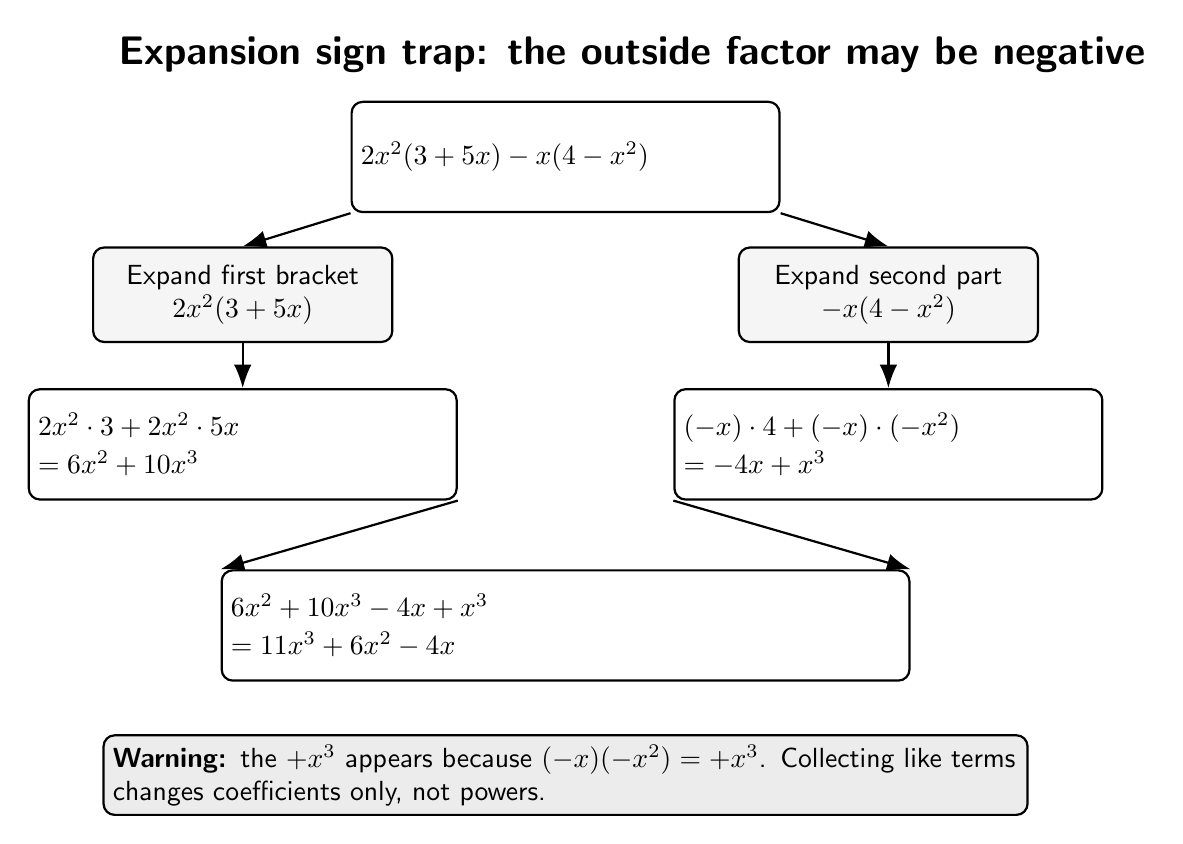
\begin{tikzpicture}[
    font=\sffamily,
    arrow/.style={-{Latex[length=3mm]}, thick},
    box/.style={draw, rounded corners=4pt, thick, fill=gray!8, align=center, minimum width=3.8cm, minimum height=1.2cm},
    work/.style={draw, rounded corners=4pt, thick, fill=white, align=left, text width=5.2cm, minimum height=1.4cm},
    warn/.style={draw, rounded corners=4pt, thick, fill=gray!15, align=left, text width=11.5cm}
]

\node[font=\sffamily\bfseries\Large, anchor=west] at (-5.8,3.7)
{Expansion sign trap: the outside factor may be negative};

\node[work] (start) at (0,2.4)
{$2x^2(3+5x)-x(4-x^2)$};

\node[box] (first) at (-4.1,0.65)
{Expand first bracket\\$2x^2(3+5x)$};

\node[box] (second) at (4.1,0.65)
{Expand second part\\$-x(4-x^2)$};

\draw[arrow] (start.south west) -- (first.north);
\draw[arrow] (start.south east) -- (second.north);

\node[work] (firstwork) at (-4.1,-1.25)
{$2x^2\cdot3+2x^2\cdot5x$\\[2pt]
$=6x^2+10x^3$};

\node[work] (secondwork) at (4.1,-1.25)
{$(-x)\cdot4+(-x)\cdot(-x^2)$\\[2pt]
$=-4x+x^3$};

\draw[arrow] (first.south) -- (firstwork.north);
\draw[arrow] (second.south) -- (secondwork.north);

\node[work, text width=8.5cm] (collect) at (0,-3.55)
{$6x^2+10x^3-4x+x^3$\\[2pt]
$=11x^3+6x^2-4x$};

\draw[arrow] (firstwork.south east) -- (collect.north west);
\draw[arrow] (secondwork.south west) -- (collect.north east);

\node[warn] at (0,-5.45)
{\textbf{Warning:} the $+x^3$ appears because $(-x)(-x^2)=+x^3$. Collecting like terms changes coefficients only, not powers.};

\end{tikzpicture}
\end{document}
